\section{\scshape Implementacja}

% ------------------------

\subsection{Wyzwania związane z implementacją logiki ewakuowanego}
\begin{frame}{Wyzwania związane z implementacją logiki ewakuowanego}
  \begin{enumerate}
    \item Dynamiczna reakcja na zagrożenie.
    \item Warunki krytyczne.
    \item Wybór wyjścia ewakuacyjnego.
  \end{enumerate}
\end{frame}

% ------------------------

\subsection{Dynamiczna reakcja na zmiany temperatury}
\begin{frame}{Dynamiczna reakcja na zmiany temperatury}
  \begin{figure}
    \centering
    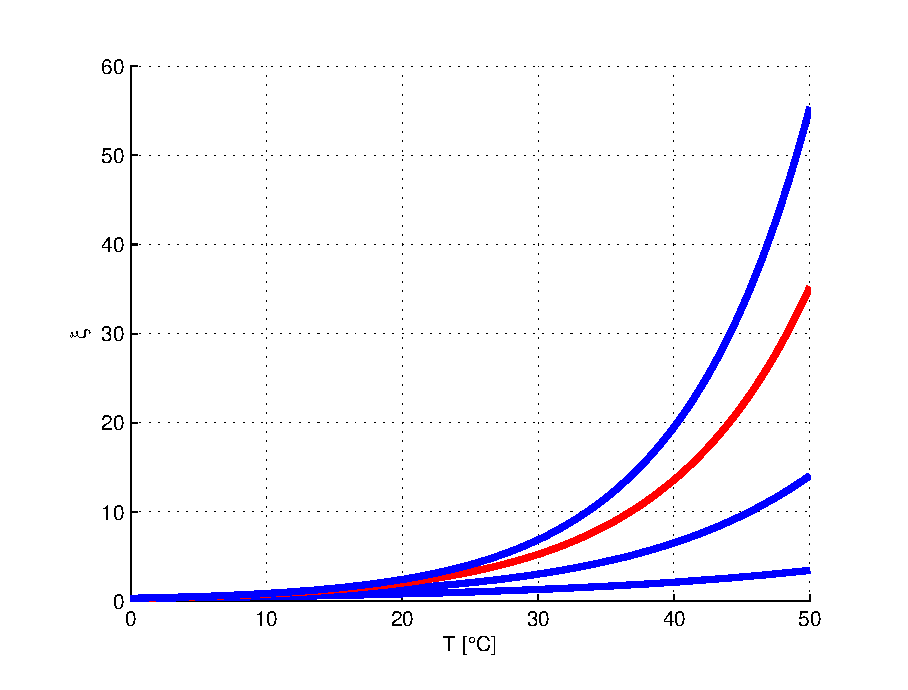
\includegraphics[height=0.6\textheight]{wykresy-kuba}
  \end{figure}
  \begin{center}
  $$\xi = \alpha \cdot B^T$$
  \end{center}
  \begin{center}
  $\alpha = 0.3$, $B = 1.1$
  \end{center}
\end{frame}

% ------------------------

\subsection{Warunki krytyczne --- stężenie CO}
\begin{frame}{Warunki krytyczne --- stężenie CO}
  \begin{figure}
    \centering
    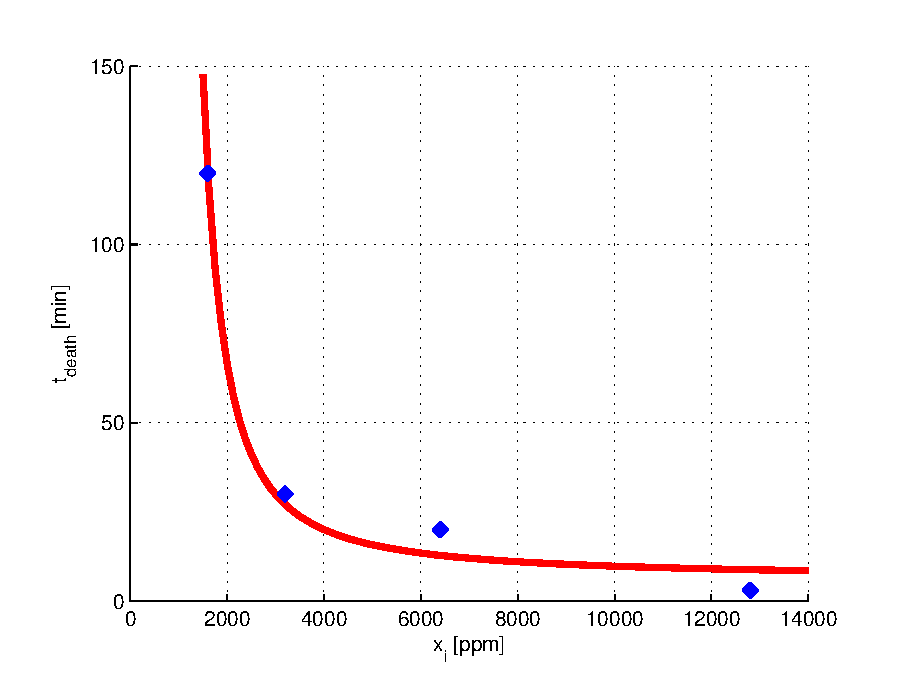
\includegraphics[height=0.6\textheight]{wykresy-wiki}
  \end{figure}
  $$HbCO_i = HbCO_{i-1} + HbCO_L \frac{CO_i}{CO_L}$$
\end{frame}